\providecommand{\main}{../../..}
\documentclass[\main/main.tex]{subfiles}

\newcommand{\paretoOne}[1]{
  \posxyzgraph{2}{4}{2*x+y<=4&&2-y<=#1}{0.25*(x-4)^2+0.25^y}
  \caption{Graph with the standard $\epsilon_2=#1$}
}

\begin{document}

\subsection{Exercise 1}
\begin{align*}
  \min f_1         & = \frac{1}{4}\rnd{x_1-4}^2 + \frac{1}{4}x^2_2 \\
  \min f_2         & = 2-x_2                                       \\
  g_1 = 2x_1 + x_2 & \leq 4                                        \\
  \bmx             & \geq \bm{0}, \bmx \in \R^2
\end{align*}

\reqPareStd{constraints methods}

\subsection{Exercise 1 resolution}
\subsubsection*{Draw the feasible regions}
Let's begin by resolving the constraint value in function of $f_1$ and $f_2$:

\begin{align*}
  x_2 & = 2- f_2                     \\
  x_1 & = \sqrt{(2- f_2)^2 - 4f_1}+4
\end{align*}
\[
  2(\sqrt{(2- f_2)^2 - 4f_1}+4) + 2-f_2 \leq 4
\]

\fig{
  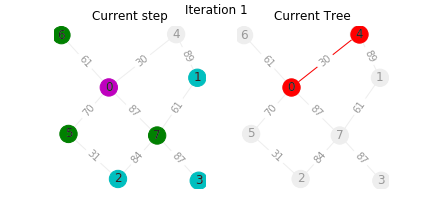
\includegraphics[width=0.9\textwidth]{pareto/1}
  \caption{Feasible region in $x_1-x_2$}
}{
  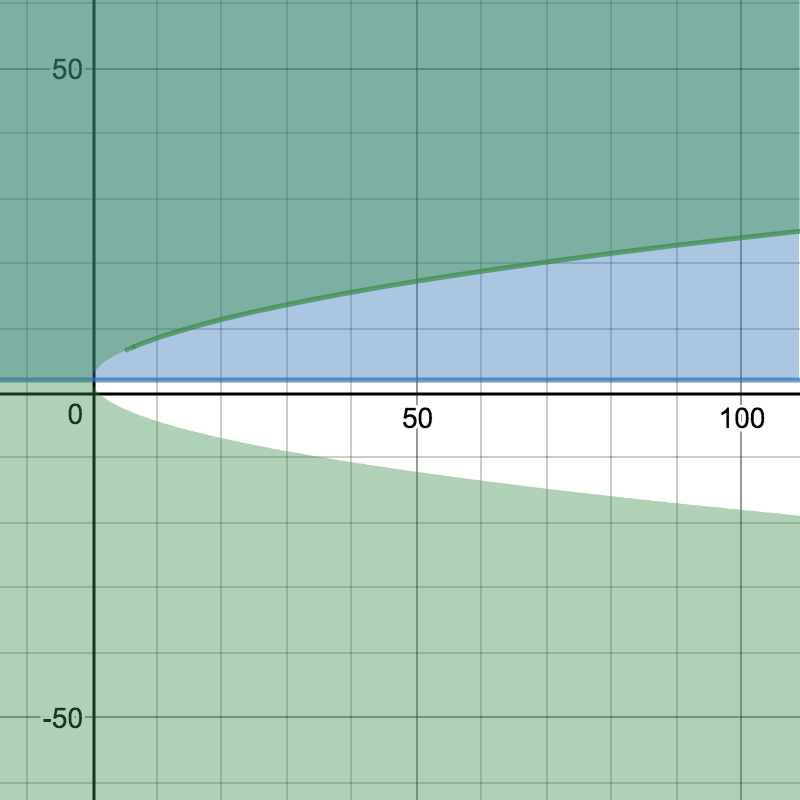
\includegraphics[width=0.9\textwidth]{pareto/1_1}
  \caption{Feasible region in $f_1-f_2$}
}

\subsubsection*{Constraints method}
Our constrain will be $f_2$, since its a minima:

\[
  f_2 = 2 - x_2 \leq \epsilon_2
\]
We begin our exploration starting at $\epsilon_2=2$
\fig{
  \paretoOne{2}
}{
  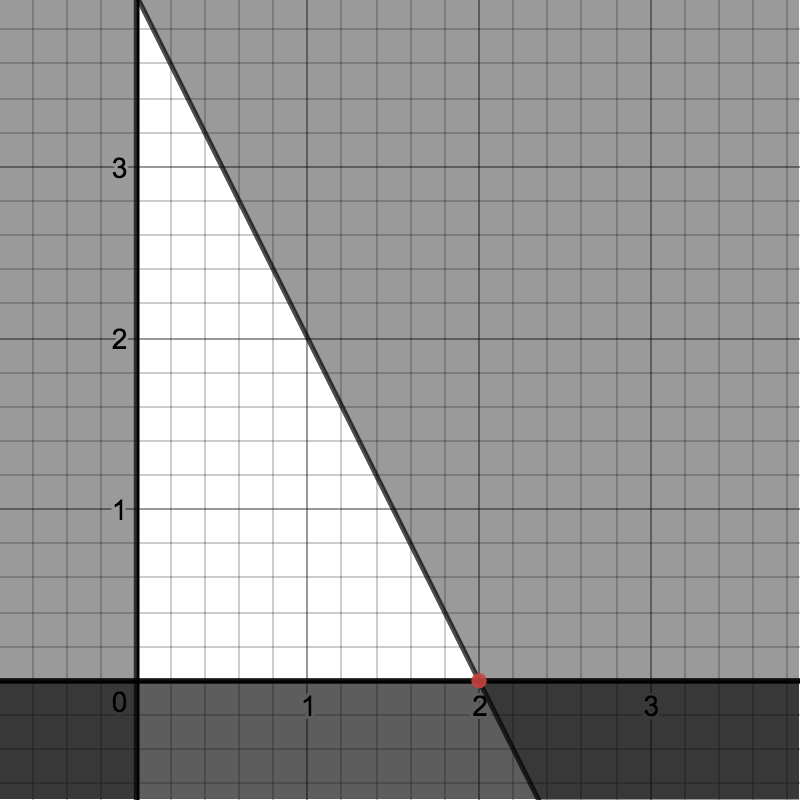
\includegraphics[width=0.9\textwidth]{pareto/1_2}
}[1]{\caption{The paretian region is the dot in $(2,0)$}}

\fig{
  \paretoOne{1}
}{
  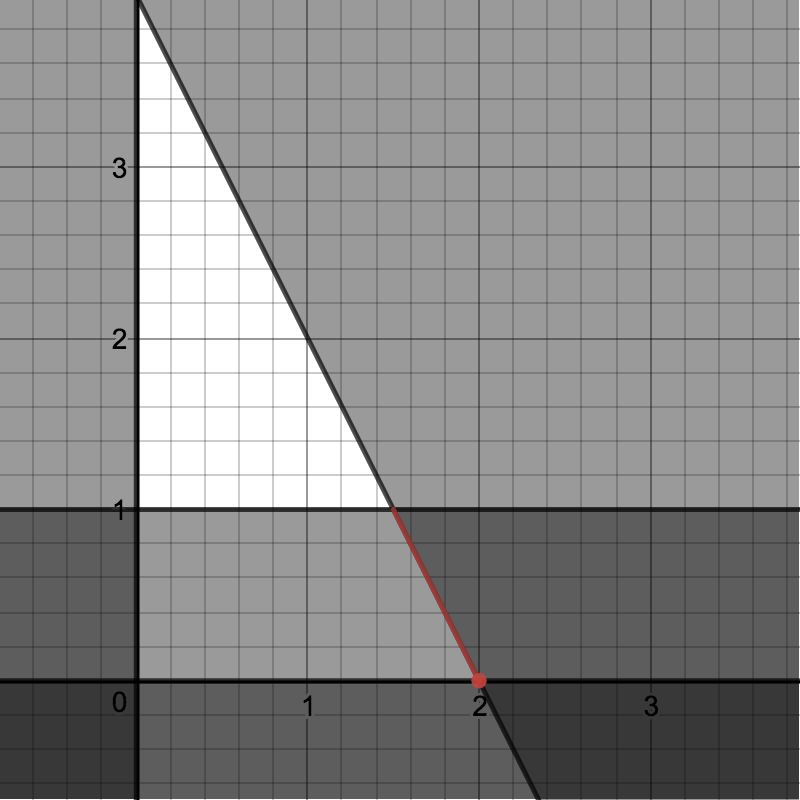
\includegraphics[width=0.9\textwidth]{pareto/1_3}
}[1]{\caption{The paretian region is the segment on the constraint $g_1$}}
\fig{
  \paretoOne{0}
}{
  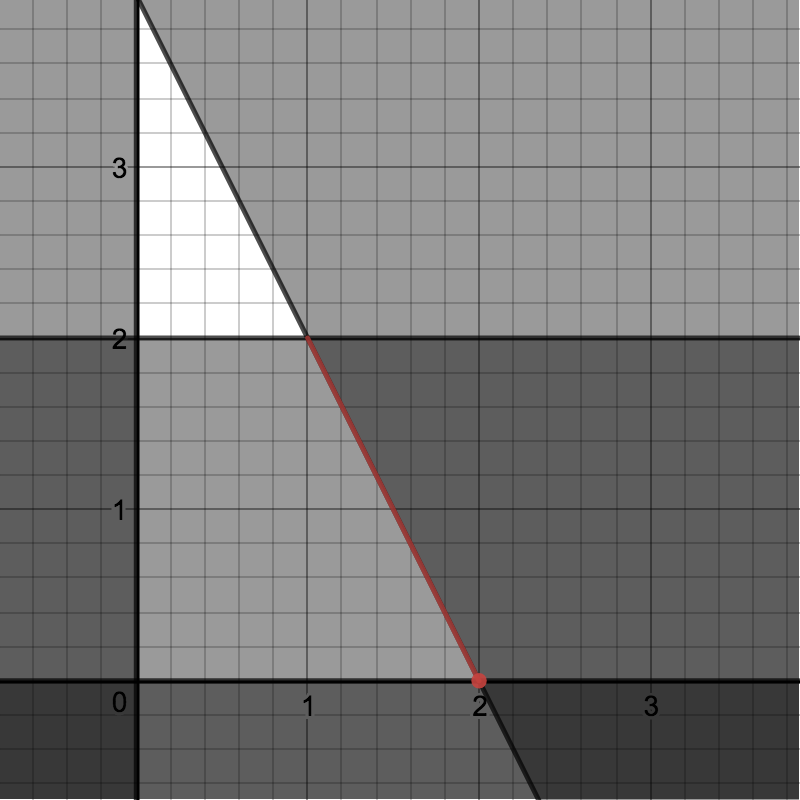
\includegraphics[width=0.9\textwidth]{pareto/1_4}
}[1]{\caption{The paretian region is the segment on the constraint $g_1$}}
\fig{
  \paretoOne{-2}
}{
  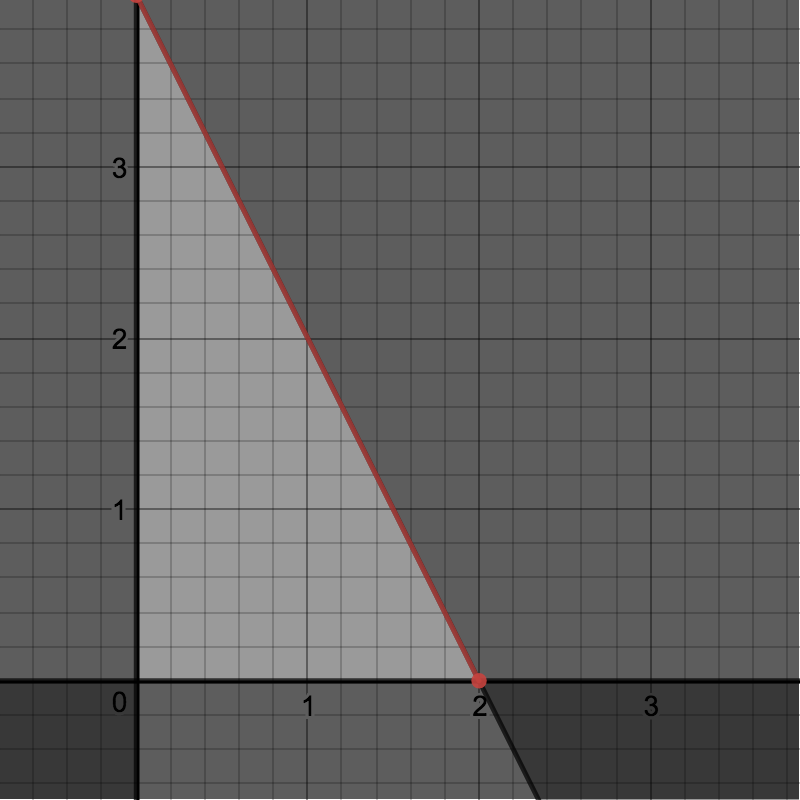
\includegraphics[width=0.9\textwidth]{pareto/1_5}
}[1]{\caption{The paretian region is the segment where $g_1$ is active and in the feasible region}}

\end{document}